\chapter{The GEM and CSC Data Acquisition Systems}
\label{chap:II-2-daq}

  The installation of GEM detectors in CMS and the integration with the CSCs require the development of a new DAQ system for the GE1/1 project. The understanding of the structure of both the GEM and CSC readout chains as well as the common CMS central DAQ is of importance in the scope of this thesis. To this end, all three systems are presented in details in the sections that follow. \\

  \section{The GE1/1 Data Acquisition System}

    \begin{figure}[h!]
      \centering
      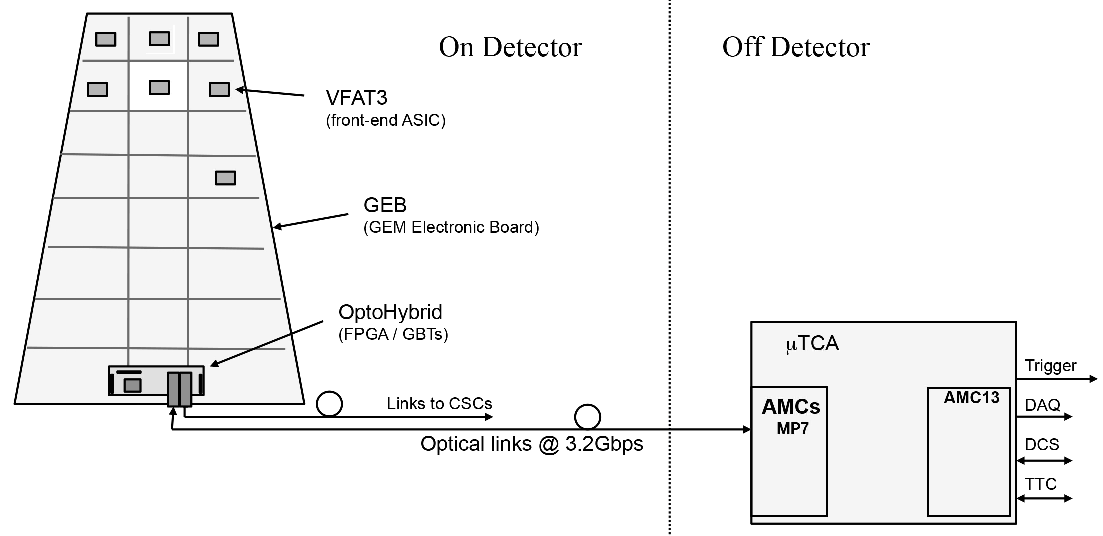
\includegraphics[width=\textwidth]{img/II-2-daq/gem-system.pdf}
      \caption{??? \cite{Colaleo:2021453}.}
      \label{fig:II-2-daq-gem-system}
    \end{figure}

    \subsection{The VFAT3 ASIC}

    \subsection{The GEM Electronics Board}

    \subsection{The OptoHybrid}

    \subsection{The GBT and Versatil Link}

    \subsection{The microTCA Standard}

    \subsection{The MP7 Advanced Mezzanine Card}

    \subsection{The AMC13}

    \subsection{The IPBus Protocol}

    \subsection{The XDAQ Application}

  \section{The CSC Data Acquisition System}

  \section{The CMS Central Data Acquisition System}
